\section{TMC6200}\label{Appendix:TMC6200}

\subsection{Standard-Schaltkreis}

\begin{figure}[H]
	\centering
	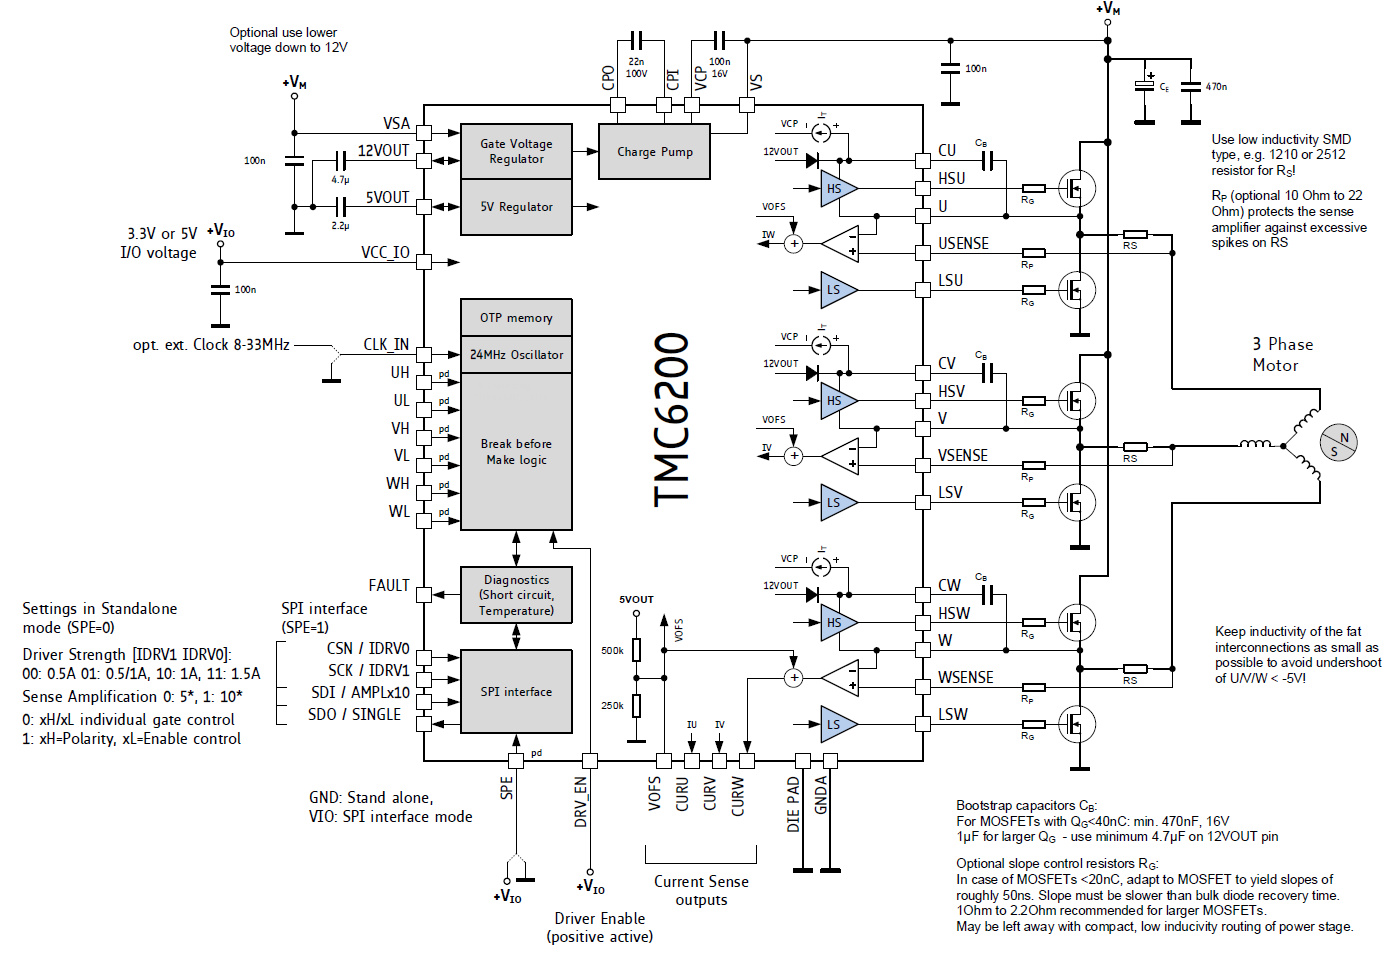
\includegraphics[width=0.8\textwidth]{graphics/Standard_Application_Cirquit_TMC6200.png}
	\caption{Standard-Anwendungs-Schaltung TMC6200.}
	\label{fig:Schaltung_TMC6200}
\end{figure}

\subsection{Blockdiagramm}

\begin{figure}[H]
	\centering
	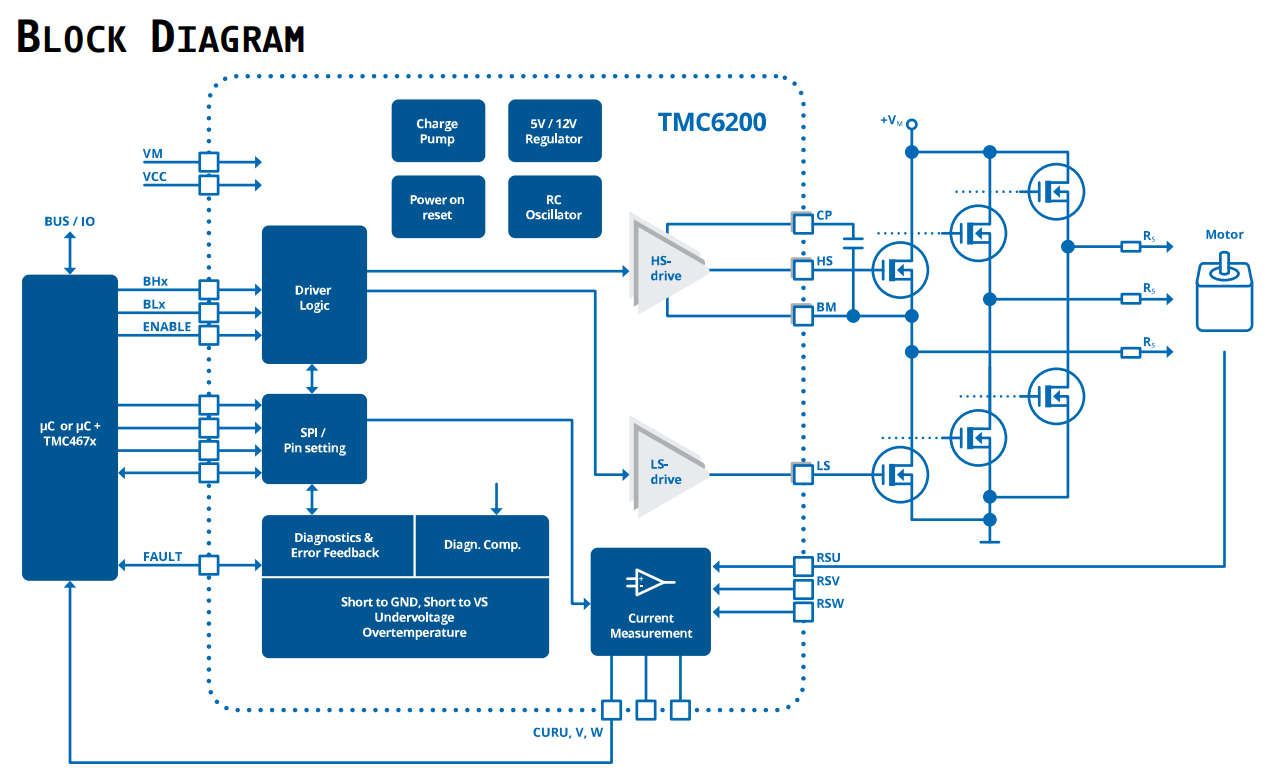
\includegraphics[width=0.8\textwidth]{graphics/Blockdiagramm_TMC6200.png}
	\caption{Blockdiagramm TMC6200.}
	\label{fig:Blockdiagramm_TMC6200}
\end{figure}

\subsection{Externe Gate-Spannungsversorgung}

\begin{figure}[H]
	\centering
	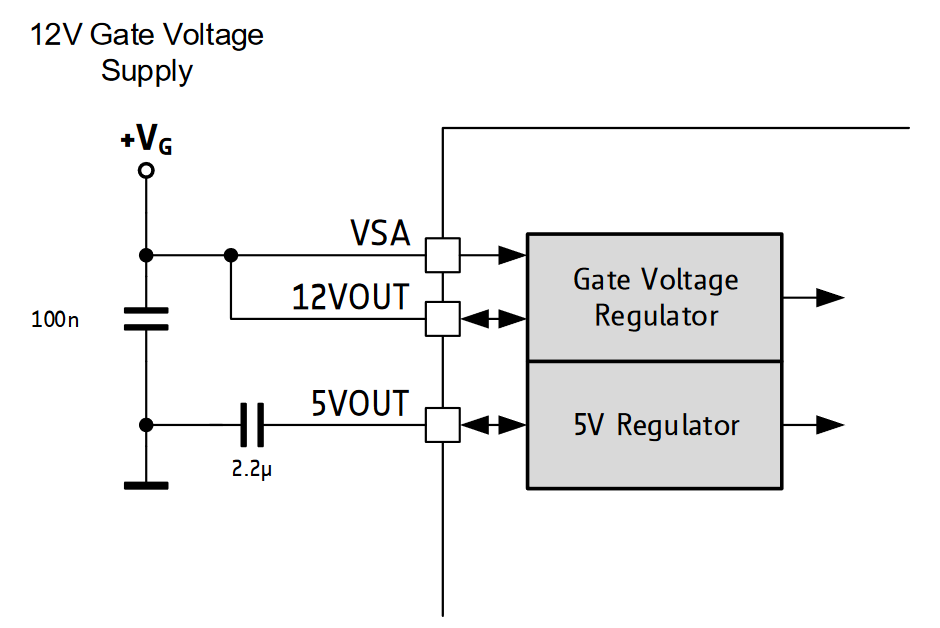
\includegraphics[width=0.4\textwidth]{graphics/Schema_Gate_Treiber_Gatespannung}
	\caption{Schema externe Gate-Spannungsversorgung.}
	\label{fig:Schema_Gate_Treiber_Gatespannung}
\end{figure}

\subsection{Inbetriebnahme}

\subsubsection{Inbetriebnahme Setup}\label{Appendix:TMC6200_Setup}

\begin{figure}[H]
	\centering
	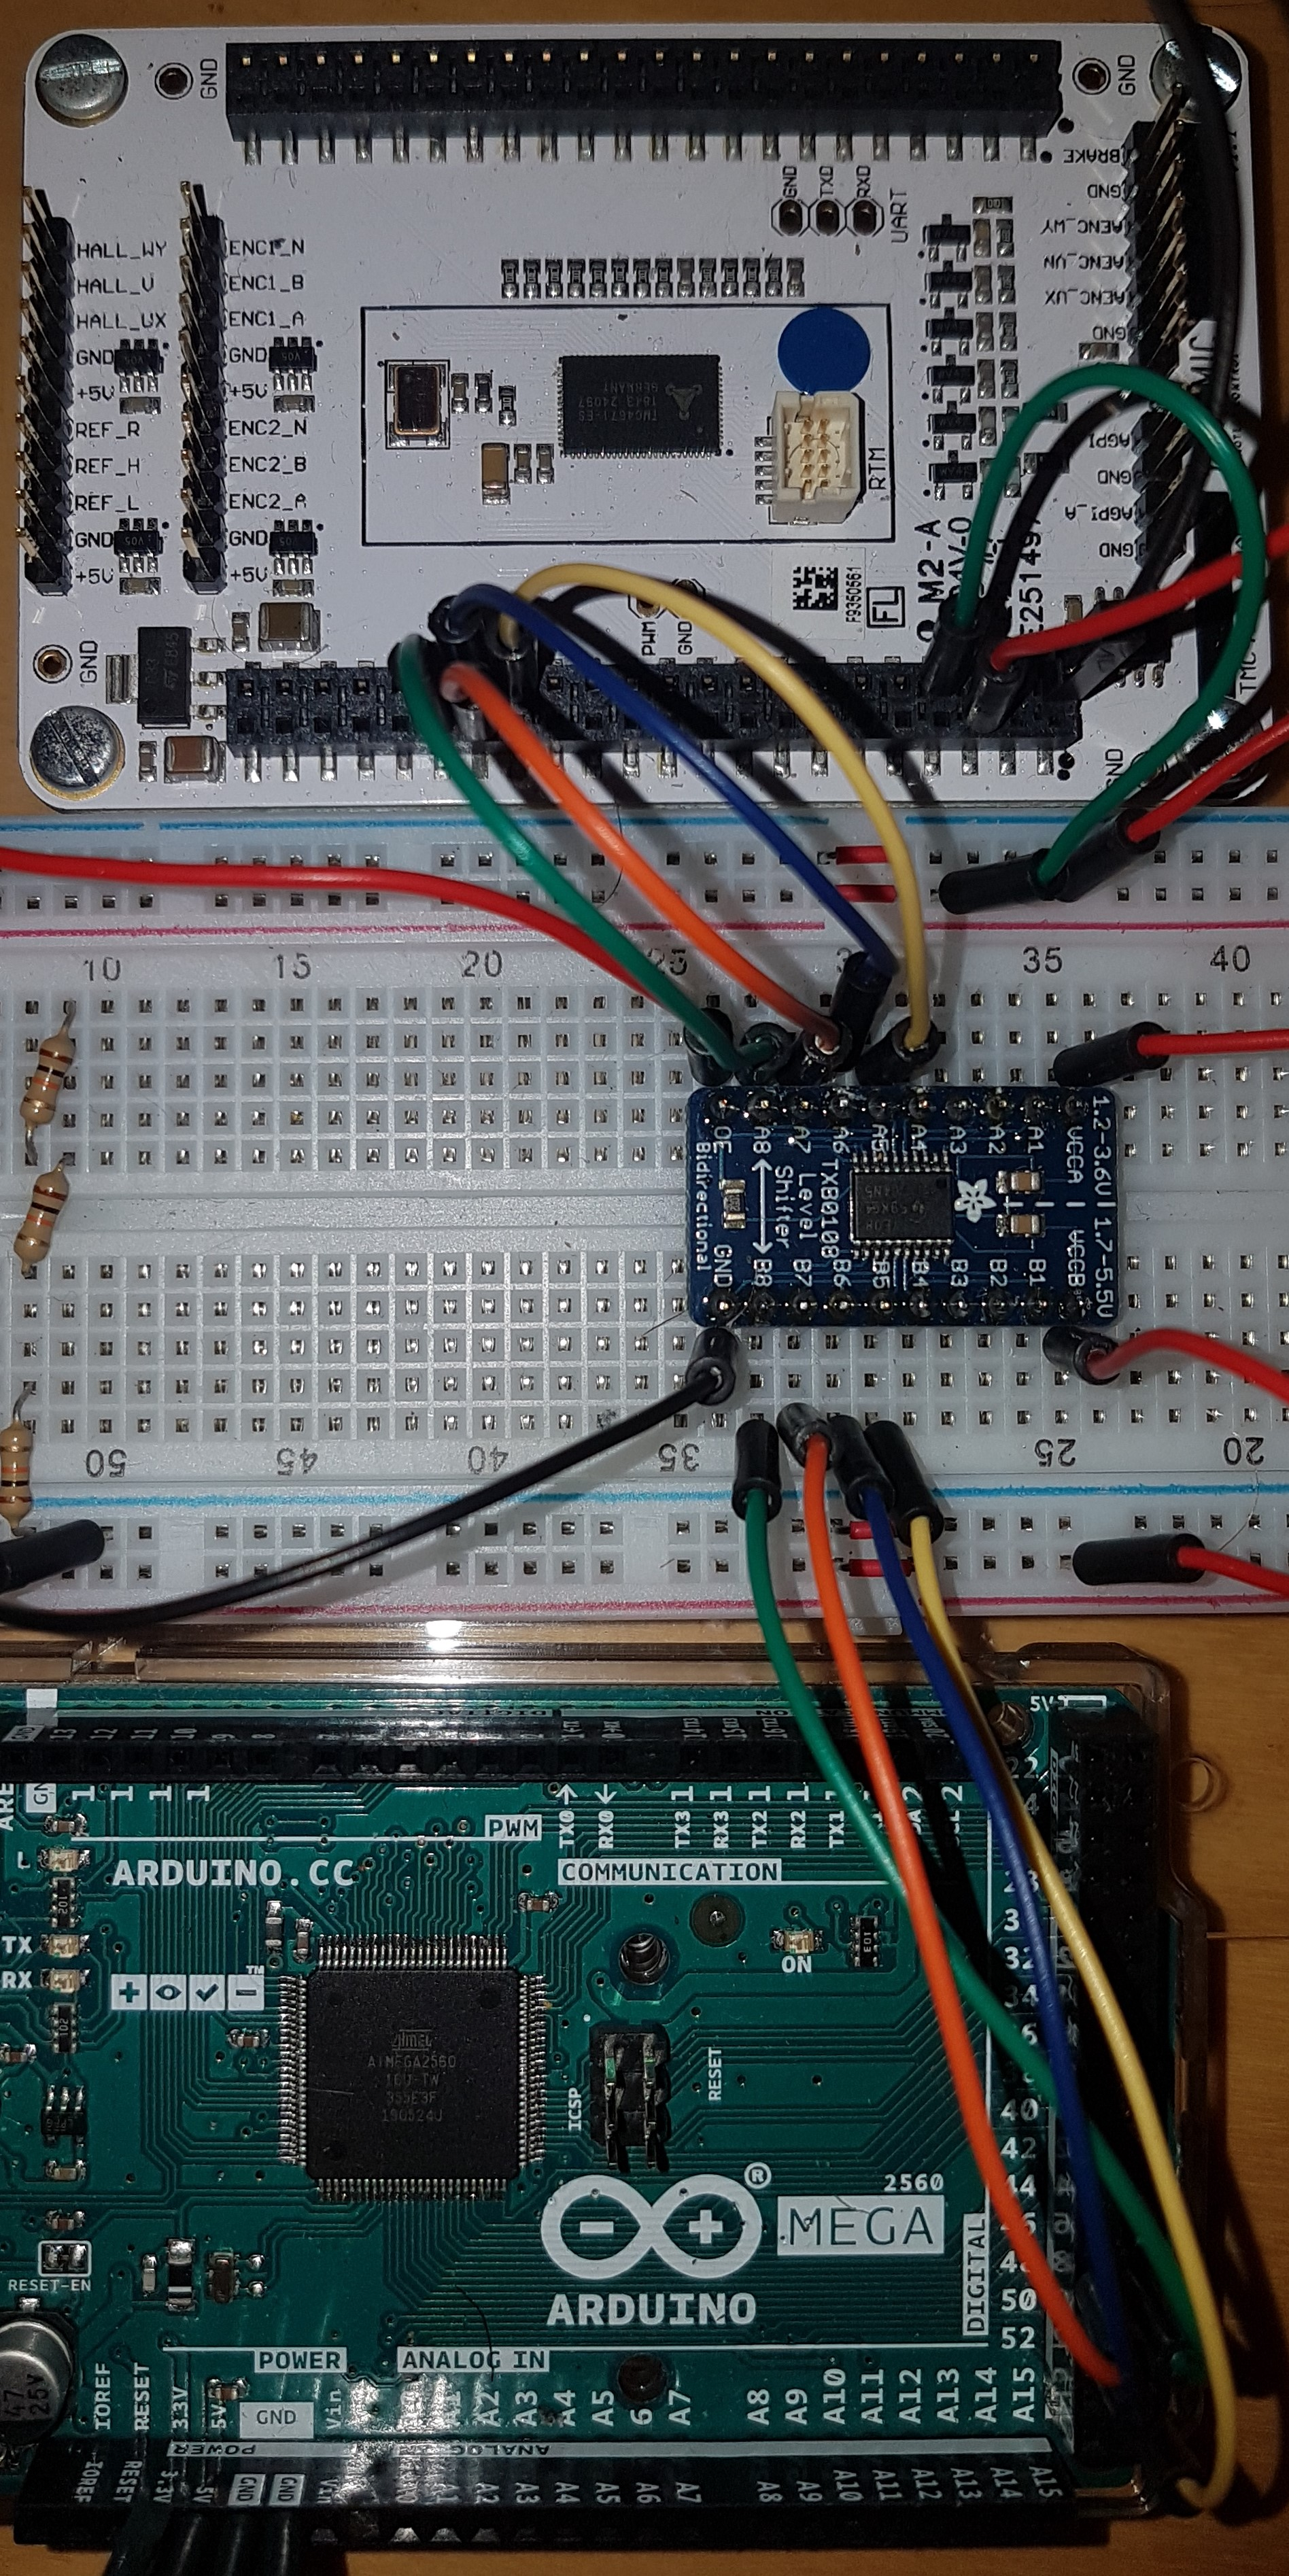
\includegraphics[angle=270,width=\textwidth]{graphics/1_komplett}
	\caption{Gesamtansicht Setup.}
	\label{fig:1_komplett}
\end{figure}

\begin{figure}[H]
	\centering
	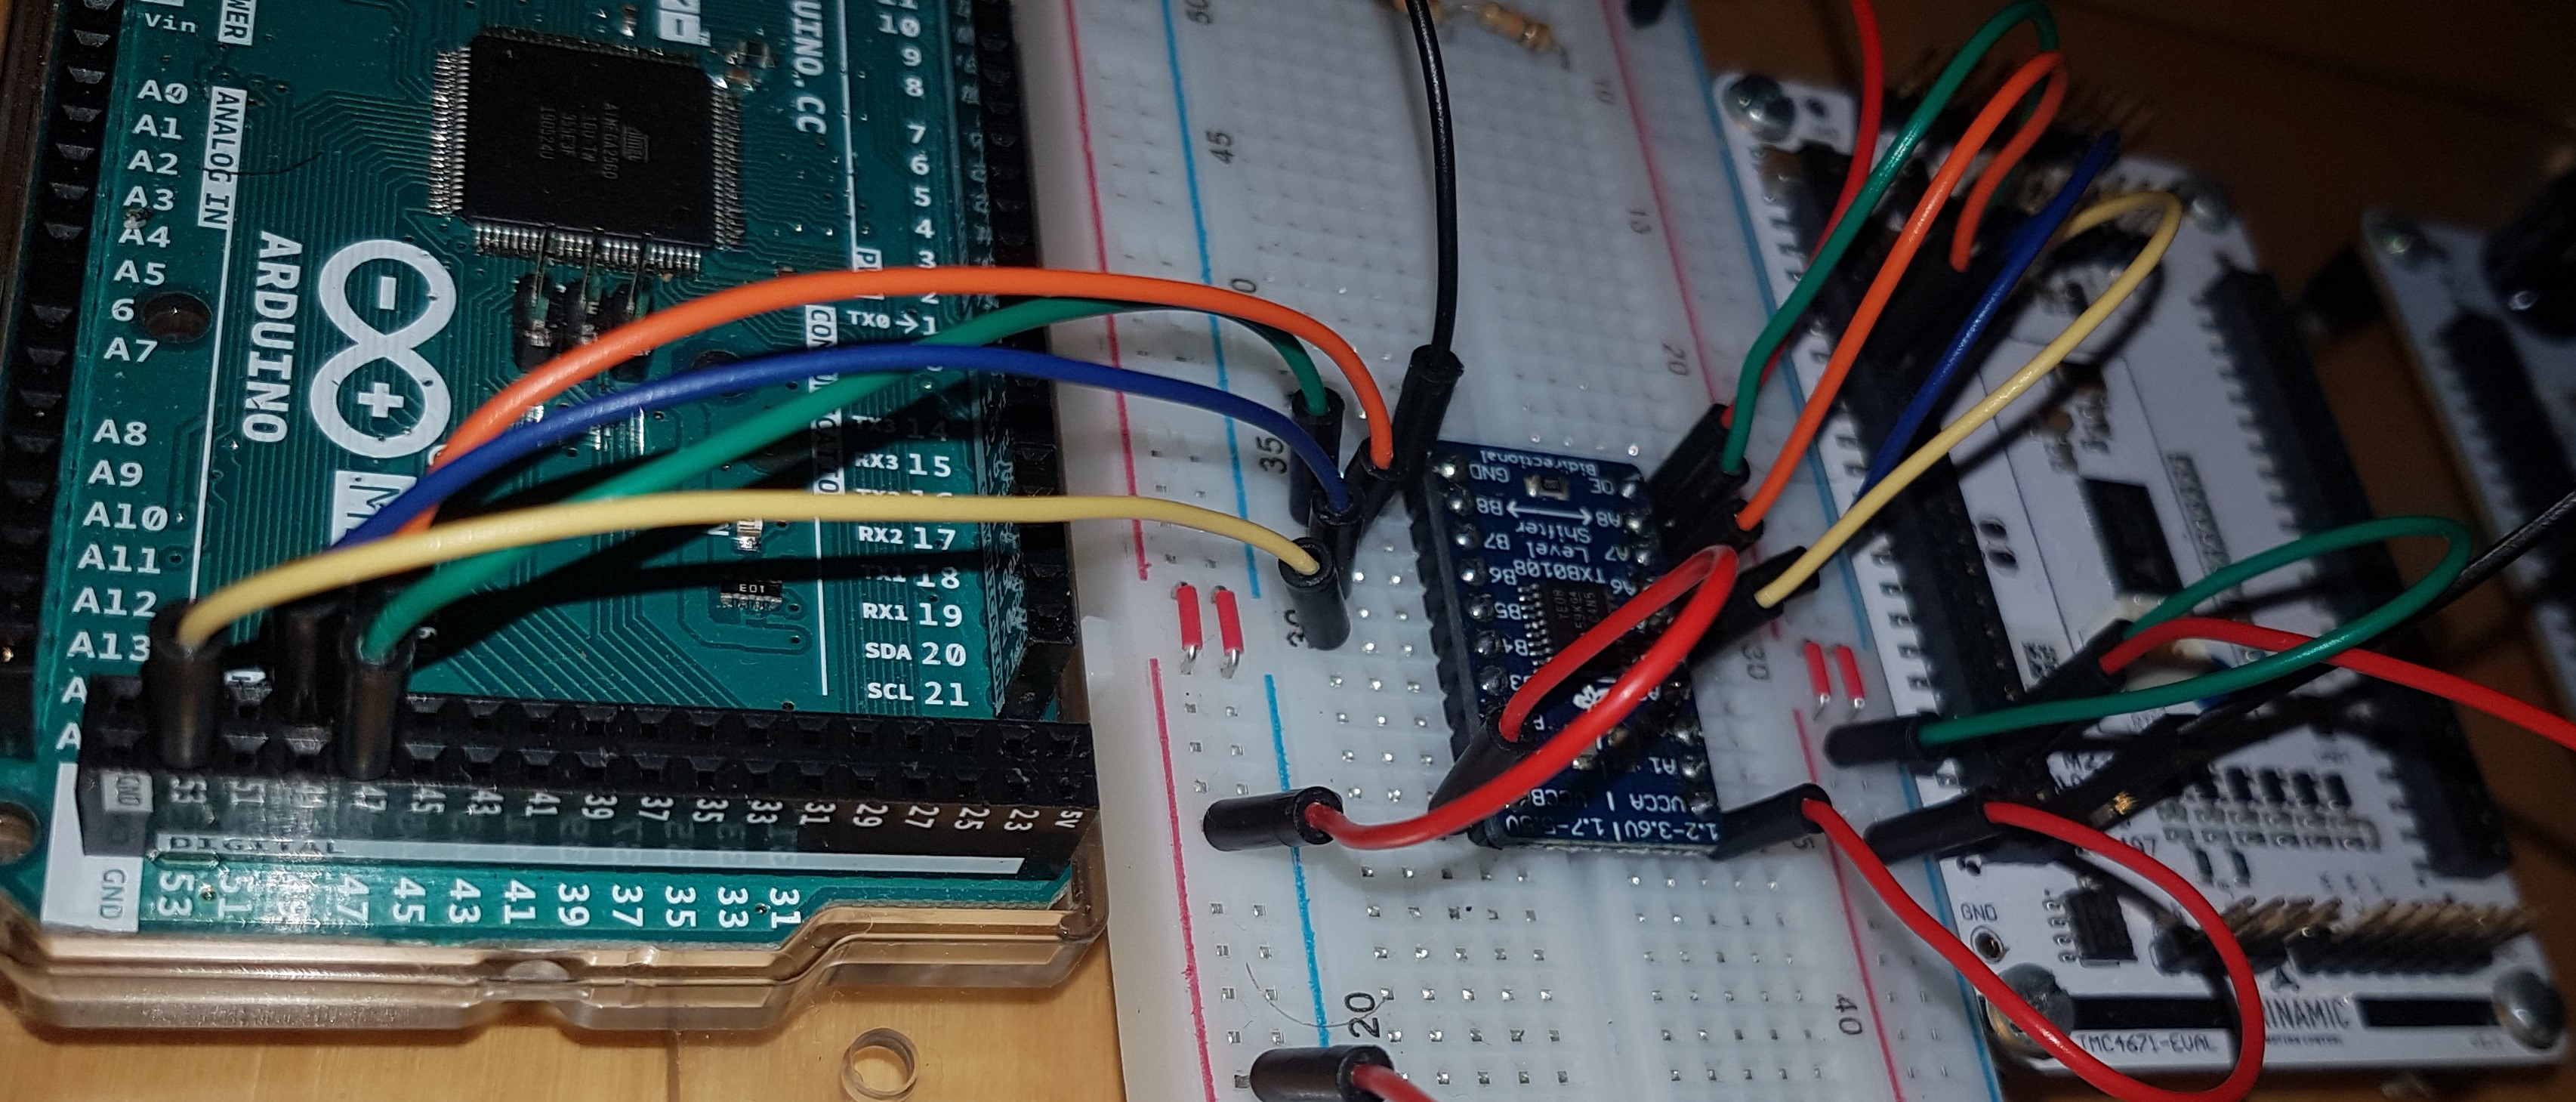
\includegraphics[width=\textwidth]{graphics/1_Arduino}
	\caption{Setup mit Fokus auf Arduino.}
	\label{fig:1_Arduino}
\end{figure}

\begin{figure}[H]
	\centering
	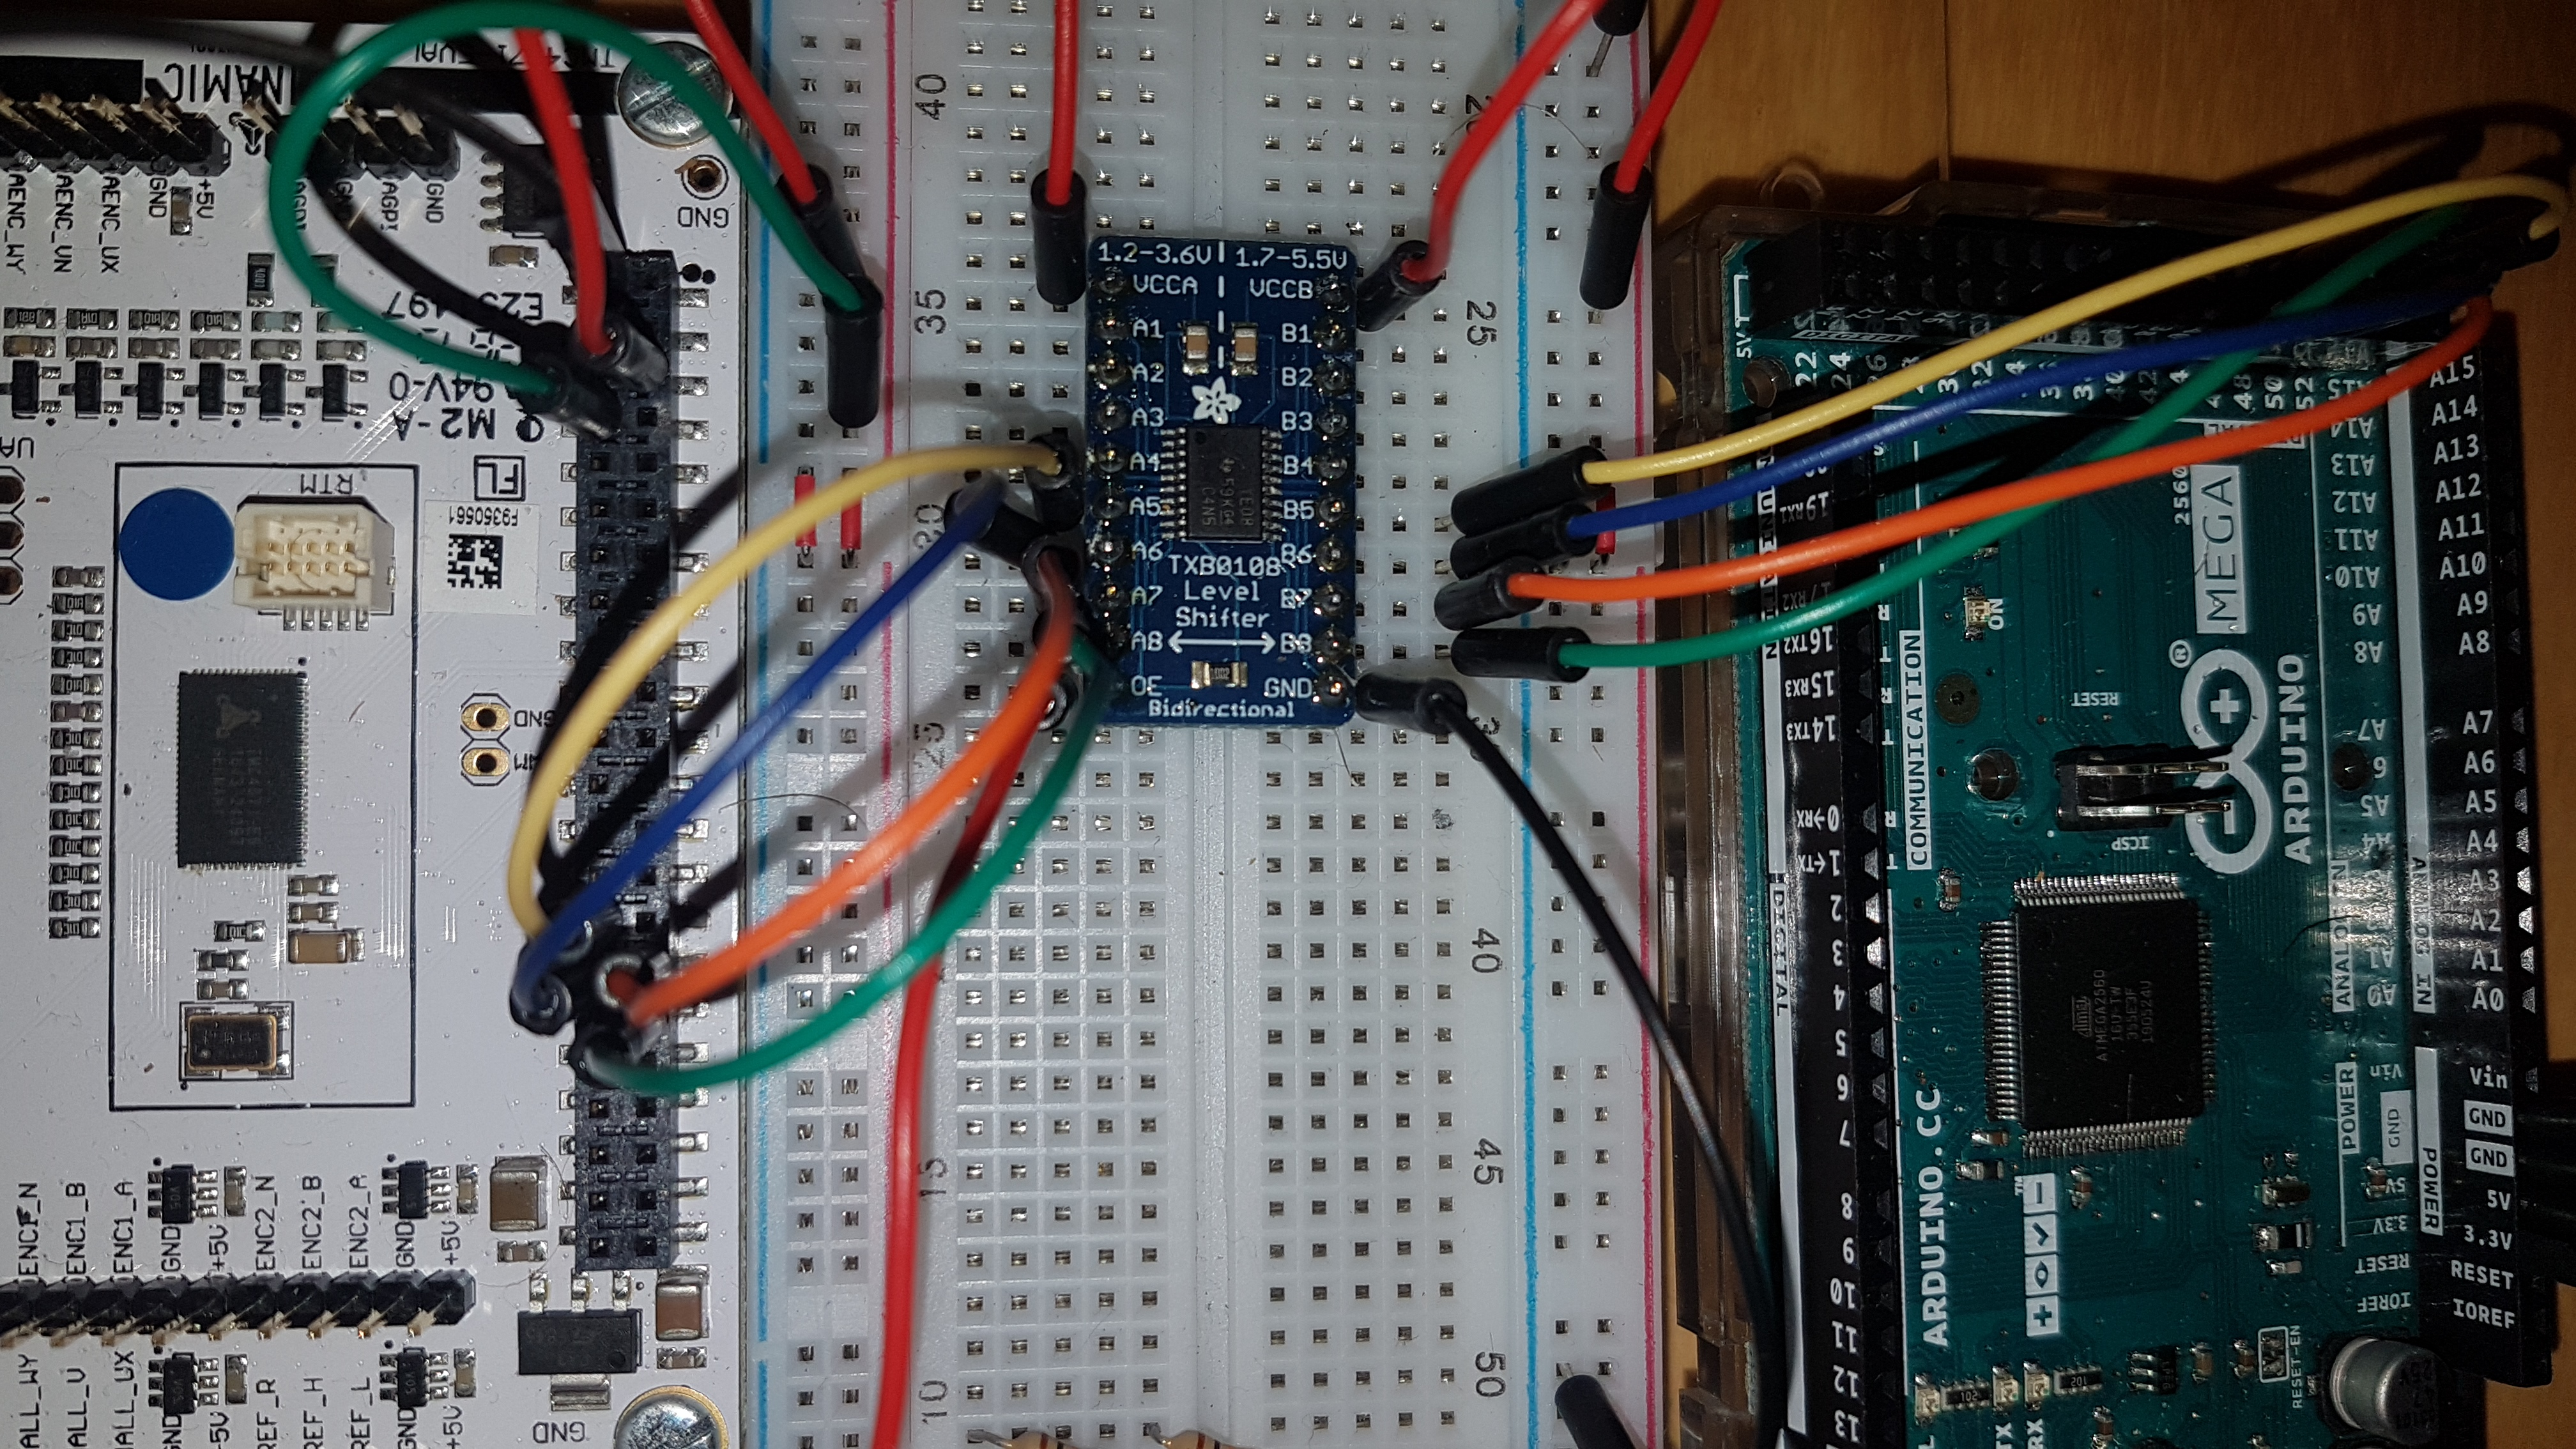
\includegraphics[angle=180,width=\textwidth]{graphics/1_EVAL}
	\caption{Setup mit Fokus auf TMC4674-EVAL.}
	\label{fig:1_EVAL}
\end{figure}

\subsubsection{Inbetriebnahme Parameter}\label{Appendix:TMC6200_SPI}

\subsubsection{Verstärkungsfaktor, Strommessung, Strommesswiderstand}

\begin{figure}[H]
	\centering
	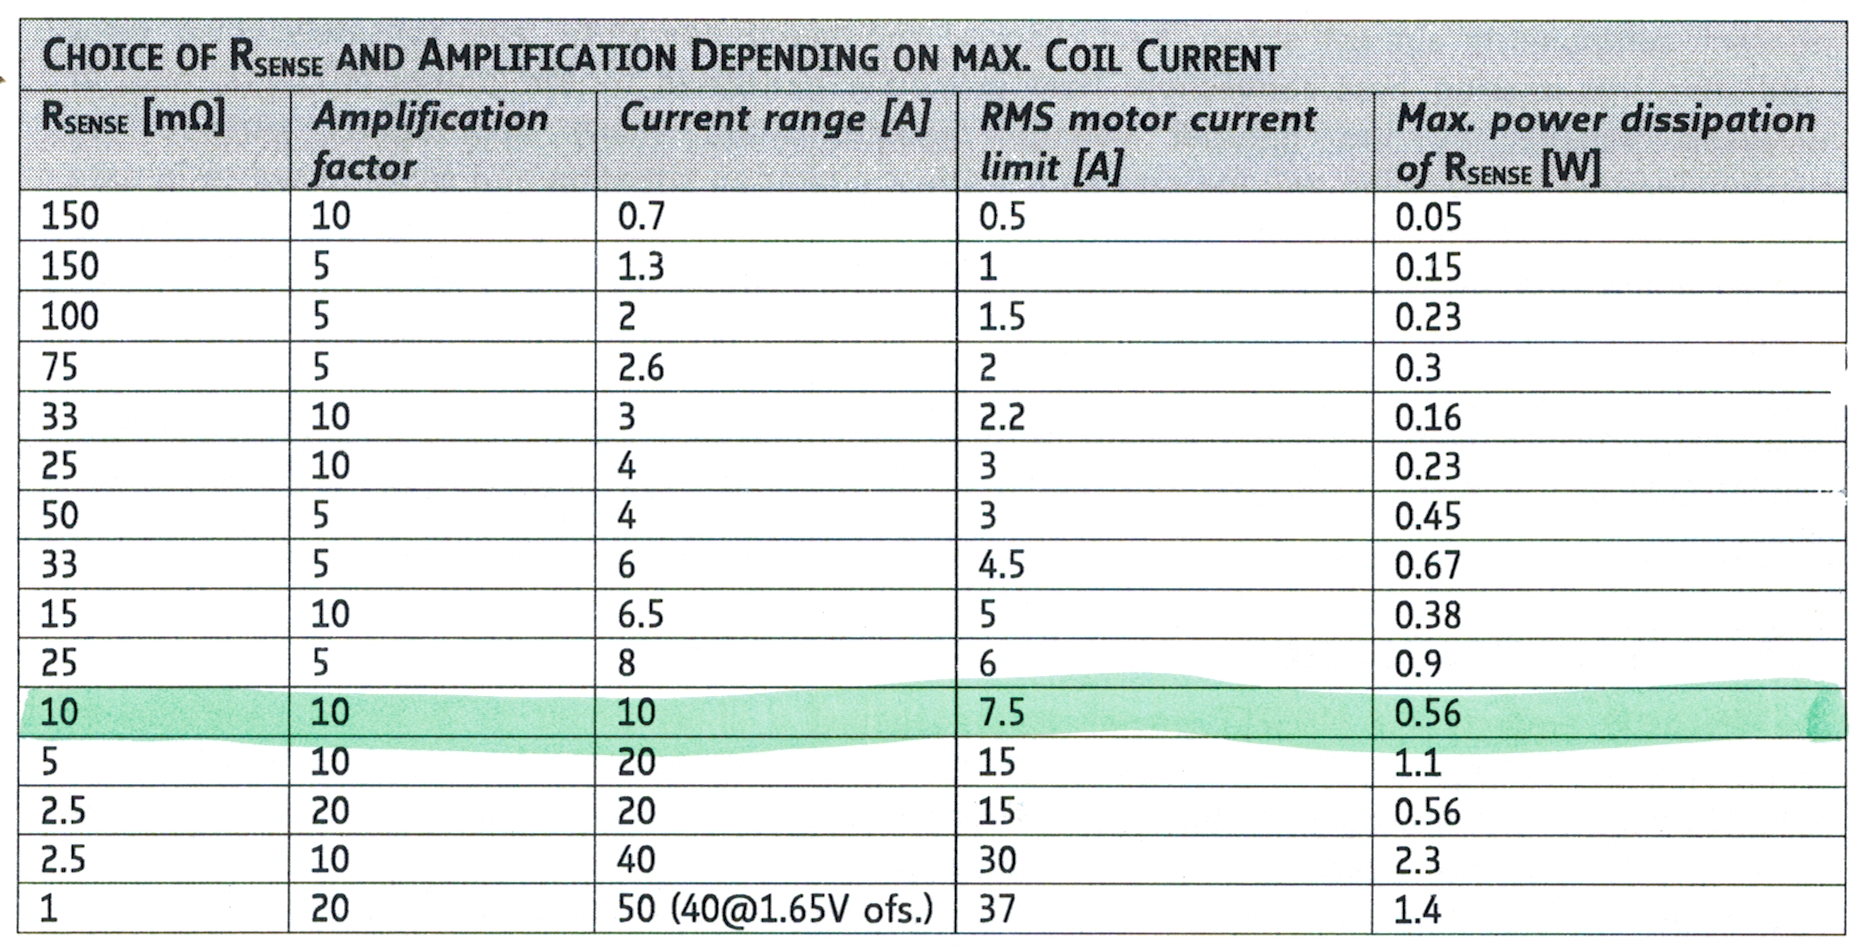
\includegraphics[width=\textwidth]{graphics/Tabelle_Shunts.png}
	\caption{Tabelle zur Bestimmung des Strommesswiderstandes aus dem Datenblatt von Trinamic.}
	\label{fig:Tabelle_Shunts}
\end{figure}

\subsubsection{Gate-Vorwiderstand}

\begin{figure}[H]
	\centering
	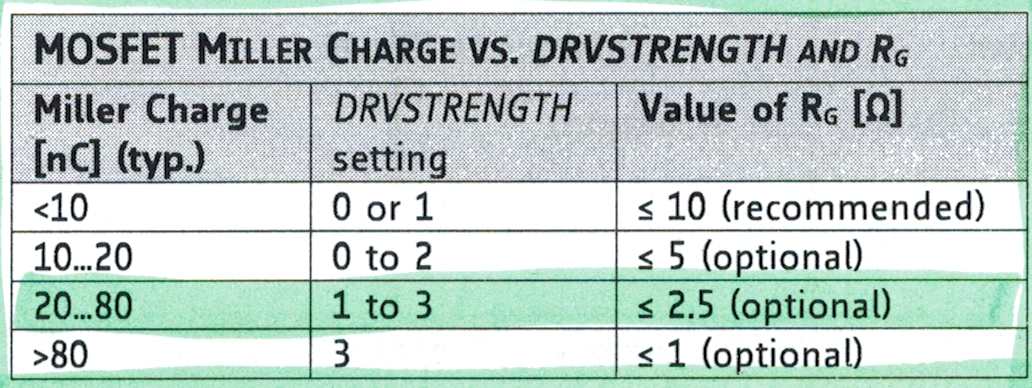
\includegraphics[width=0.5\textwidth]{graphics/Tabelle_Gatewiderstaende.png}
	\caption{Tabelle zur Bestimmung der Gatewiderstände aus dem Datenblatt von Trinamic.}
	\label{fig:Tabelle_Gatewiderstaende}
\end{figure}

\subsubsection{Inbetriebnahme SPI-Kommunikation}\label{Appendix:TMC6200_SPI}

\begin{figure}[H]
\center
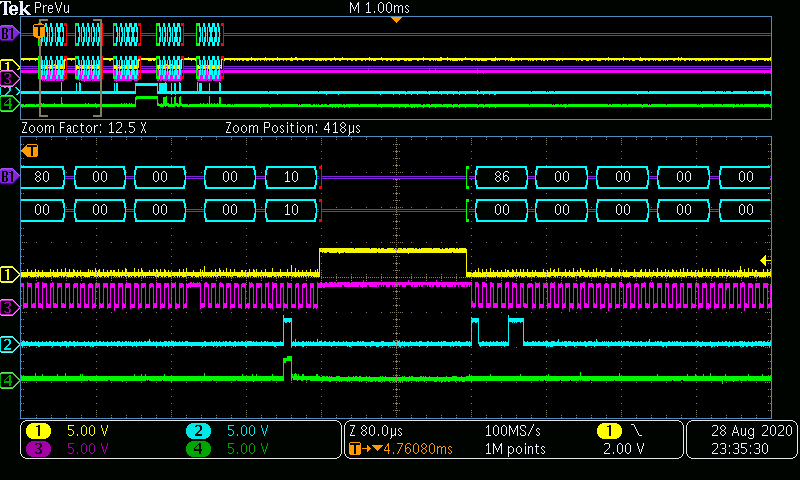
\includegraphics[width = \textwidth]{graphics/TMC6200_Beschreiben2}
\caption{SPI-Übertragung Write 1.}
\label{fig:TMC6200_Beschreiben2}
\end{figure}

\begin{figure}[H]
\center
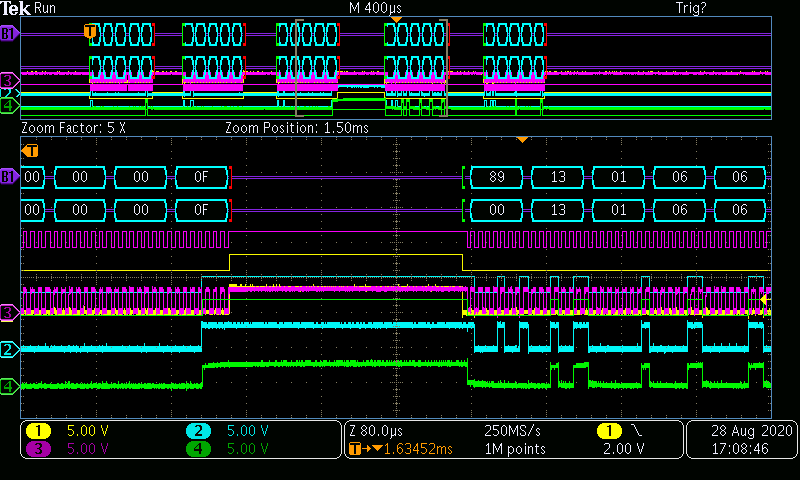
\includegraphics[width = \textwidth]{graphics/TMC6200_Beschreiben}
\caption{SPI-Übertragung Write 2.}
\label{fig:TMC6200_Beschreiben}
\end{figure}

\begin{figure}[H]
\center
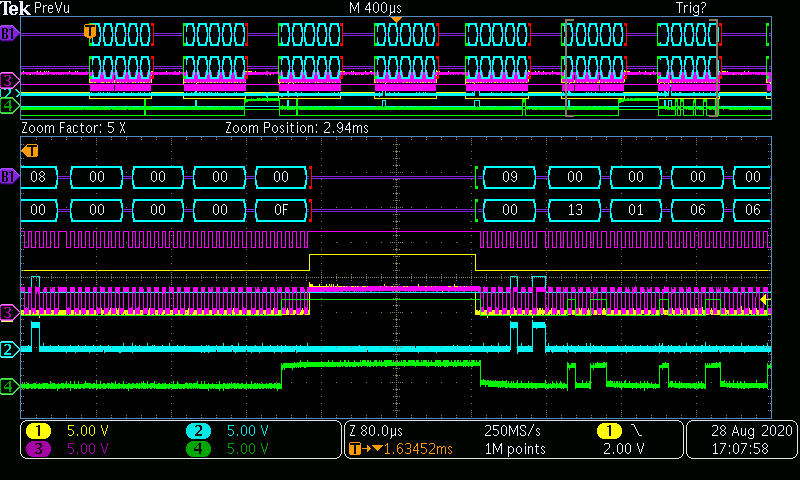
\includegraphics[width = \textwidth]{graphics/TMC6200_Lesen}
\caption{SPI-Übertragung Read.}
\label{fig:TMC6200_Lesen}
\end{figure}

\begin{figure}[H]
\center
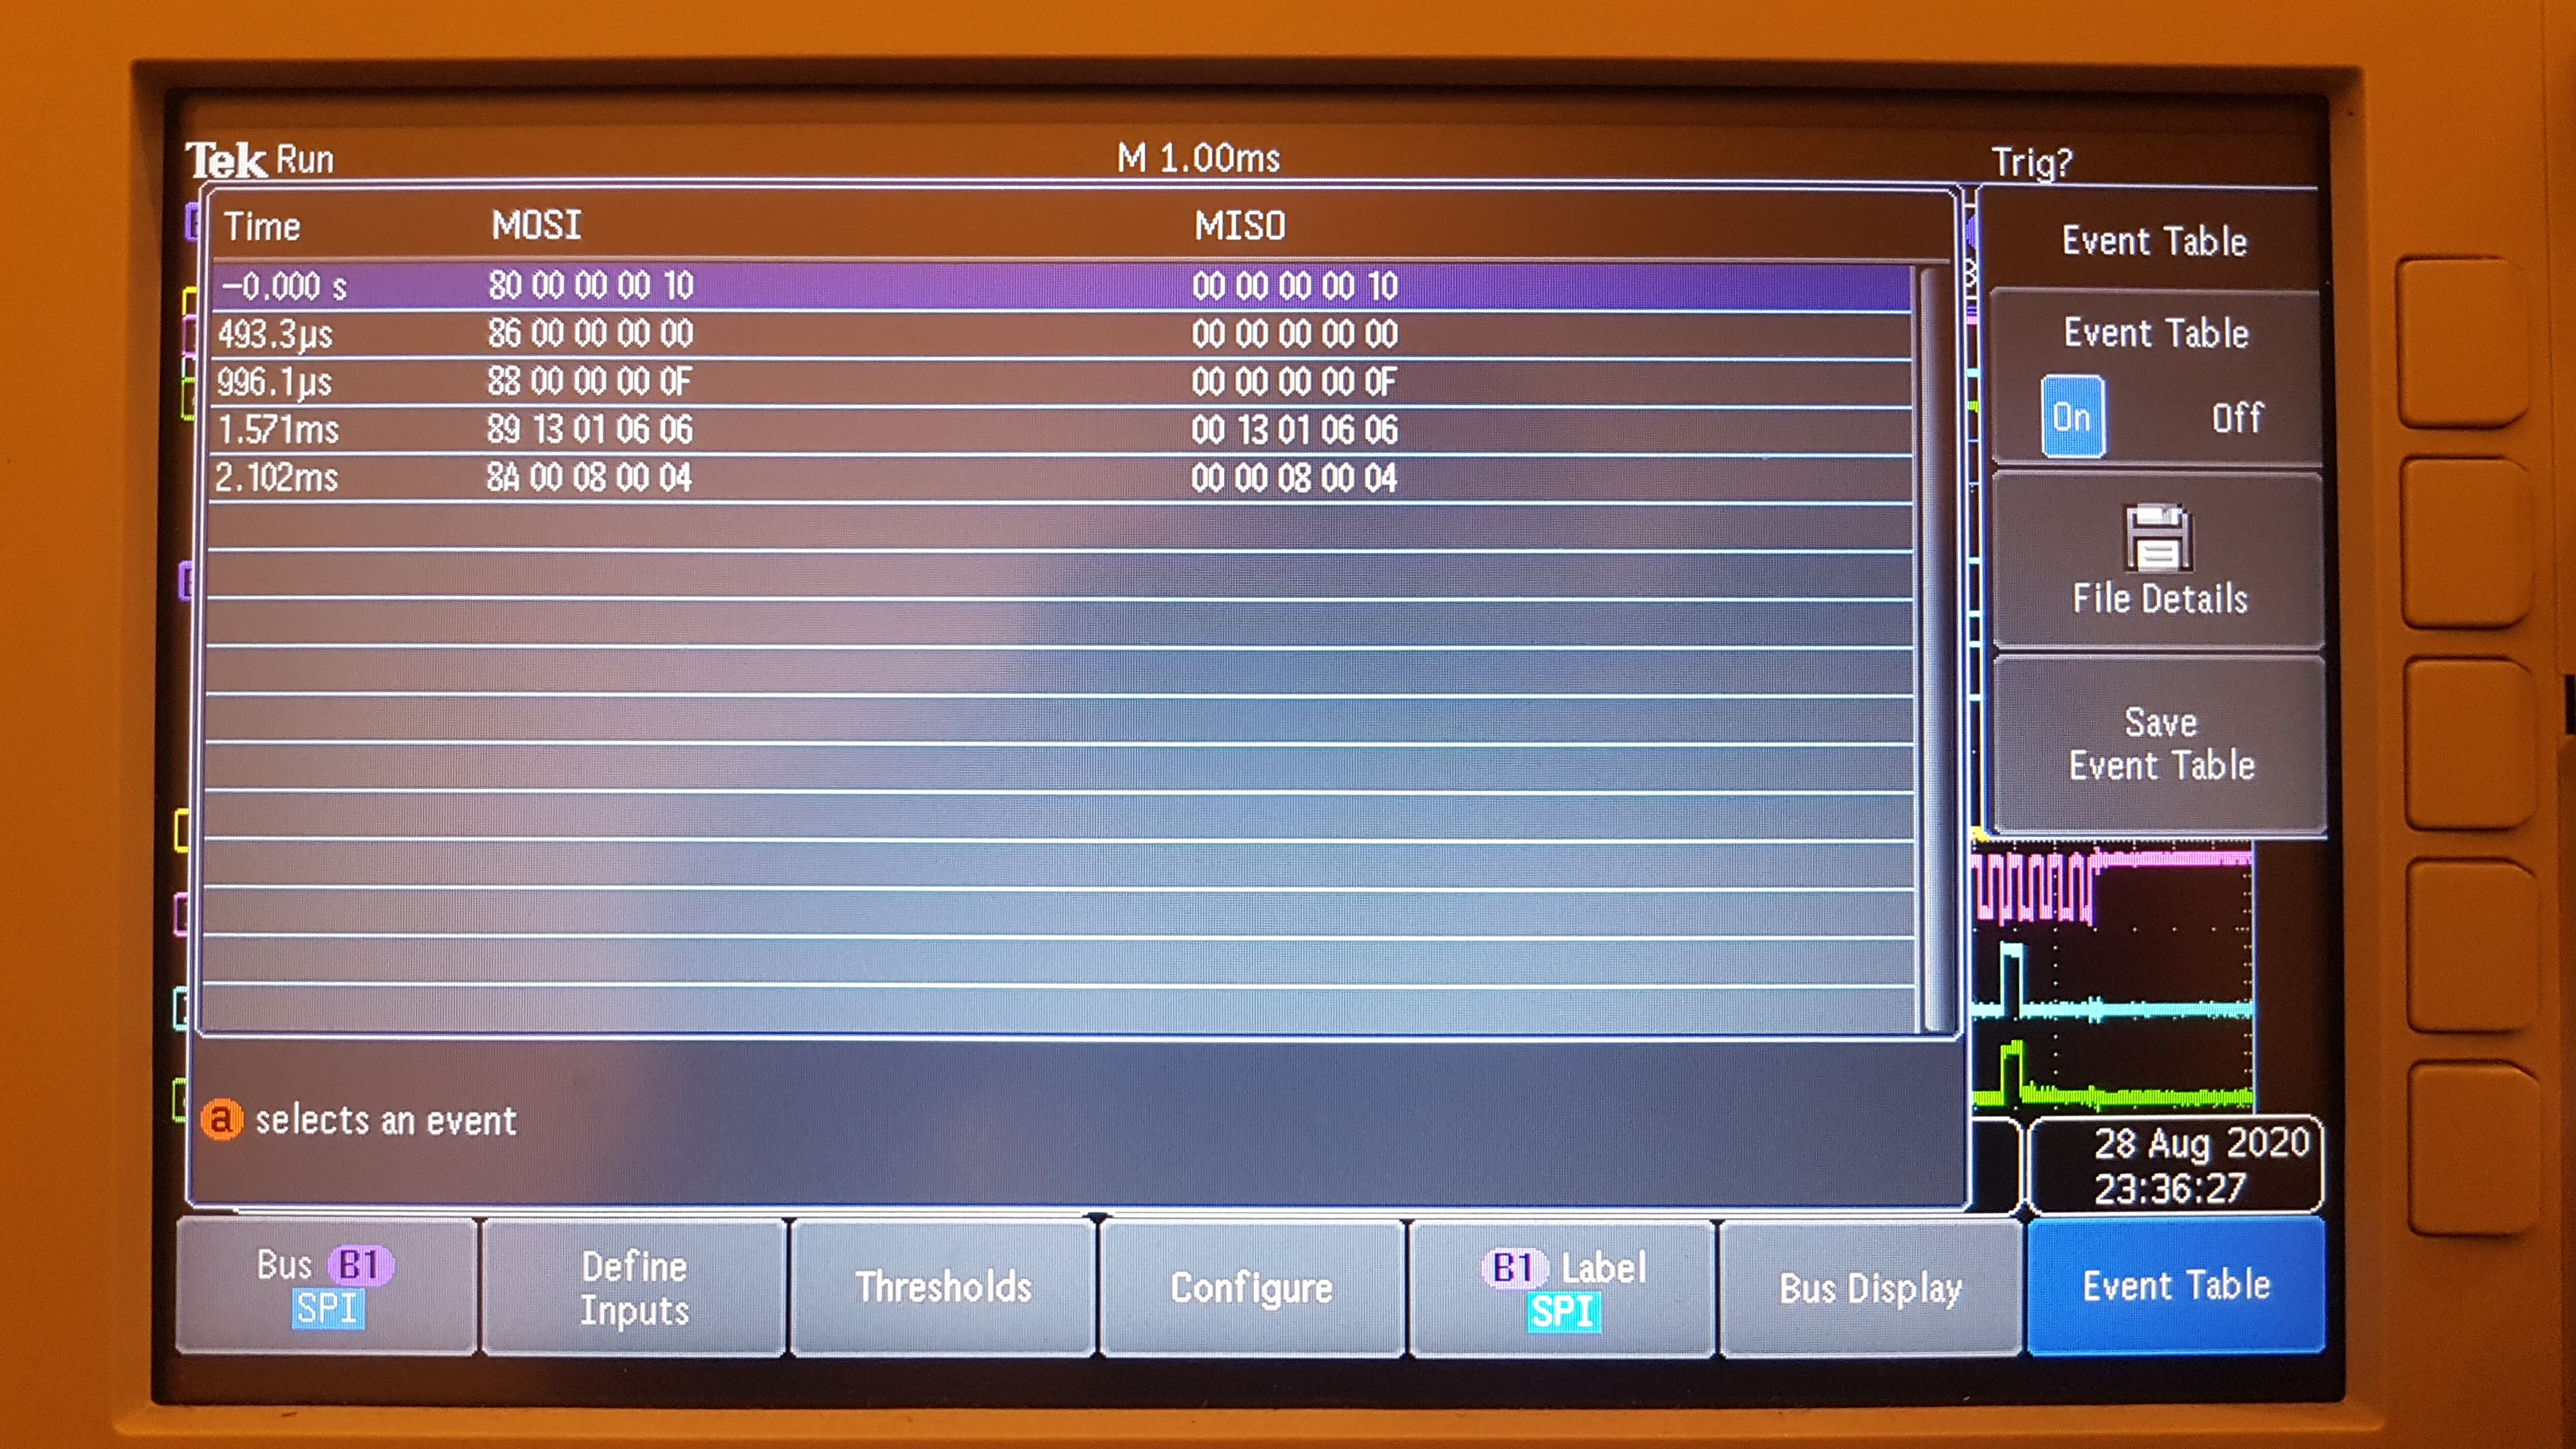
\includegraphics[width = \textwidth]{graphics/TMC6200_EventTable_Beschreiben_Bild}
\caption{Event-Table Inbetriebnahme TMC6200.}
\label{fig:TMC6200_EventTable_Beschreiben_Bild}
\end{figure}

\begin{figure}[H]
\center
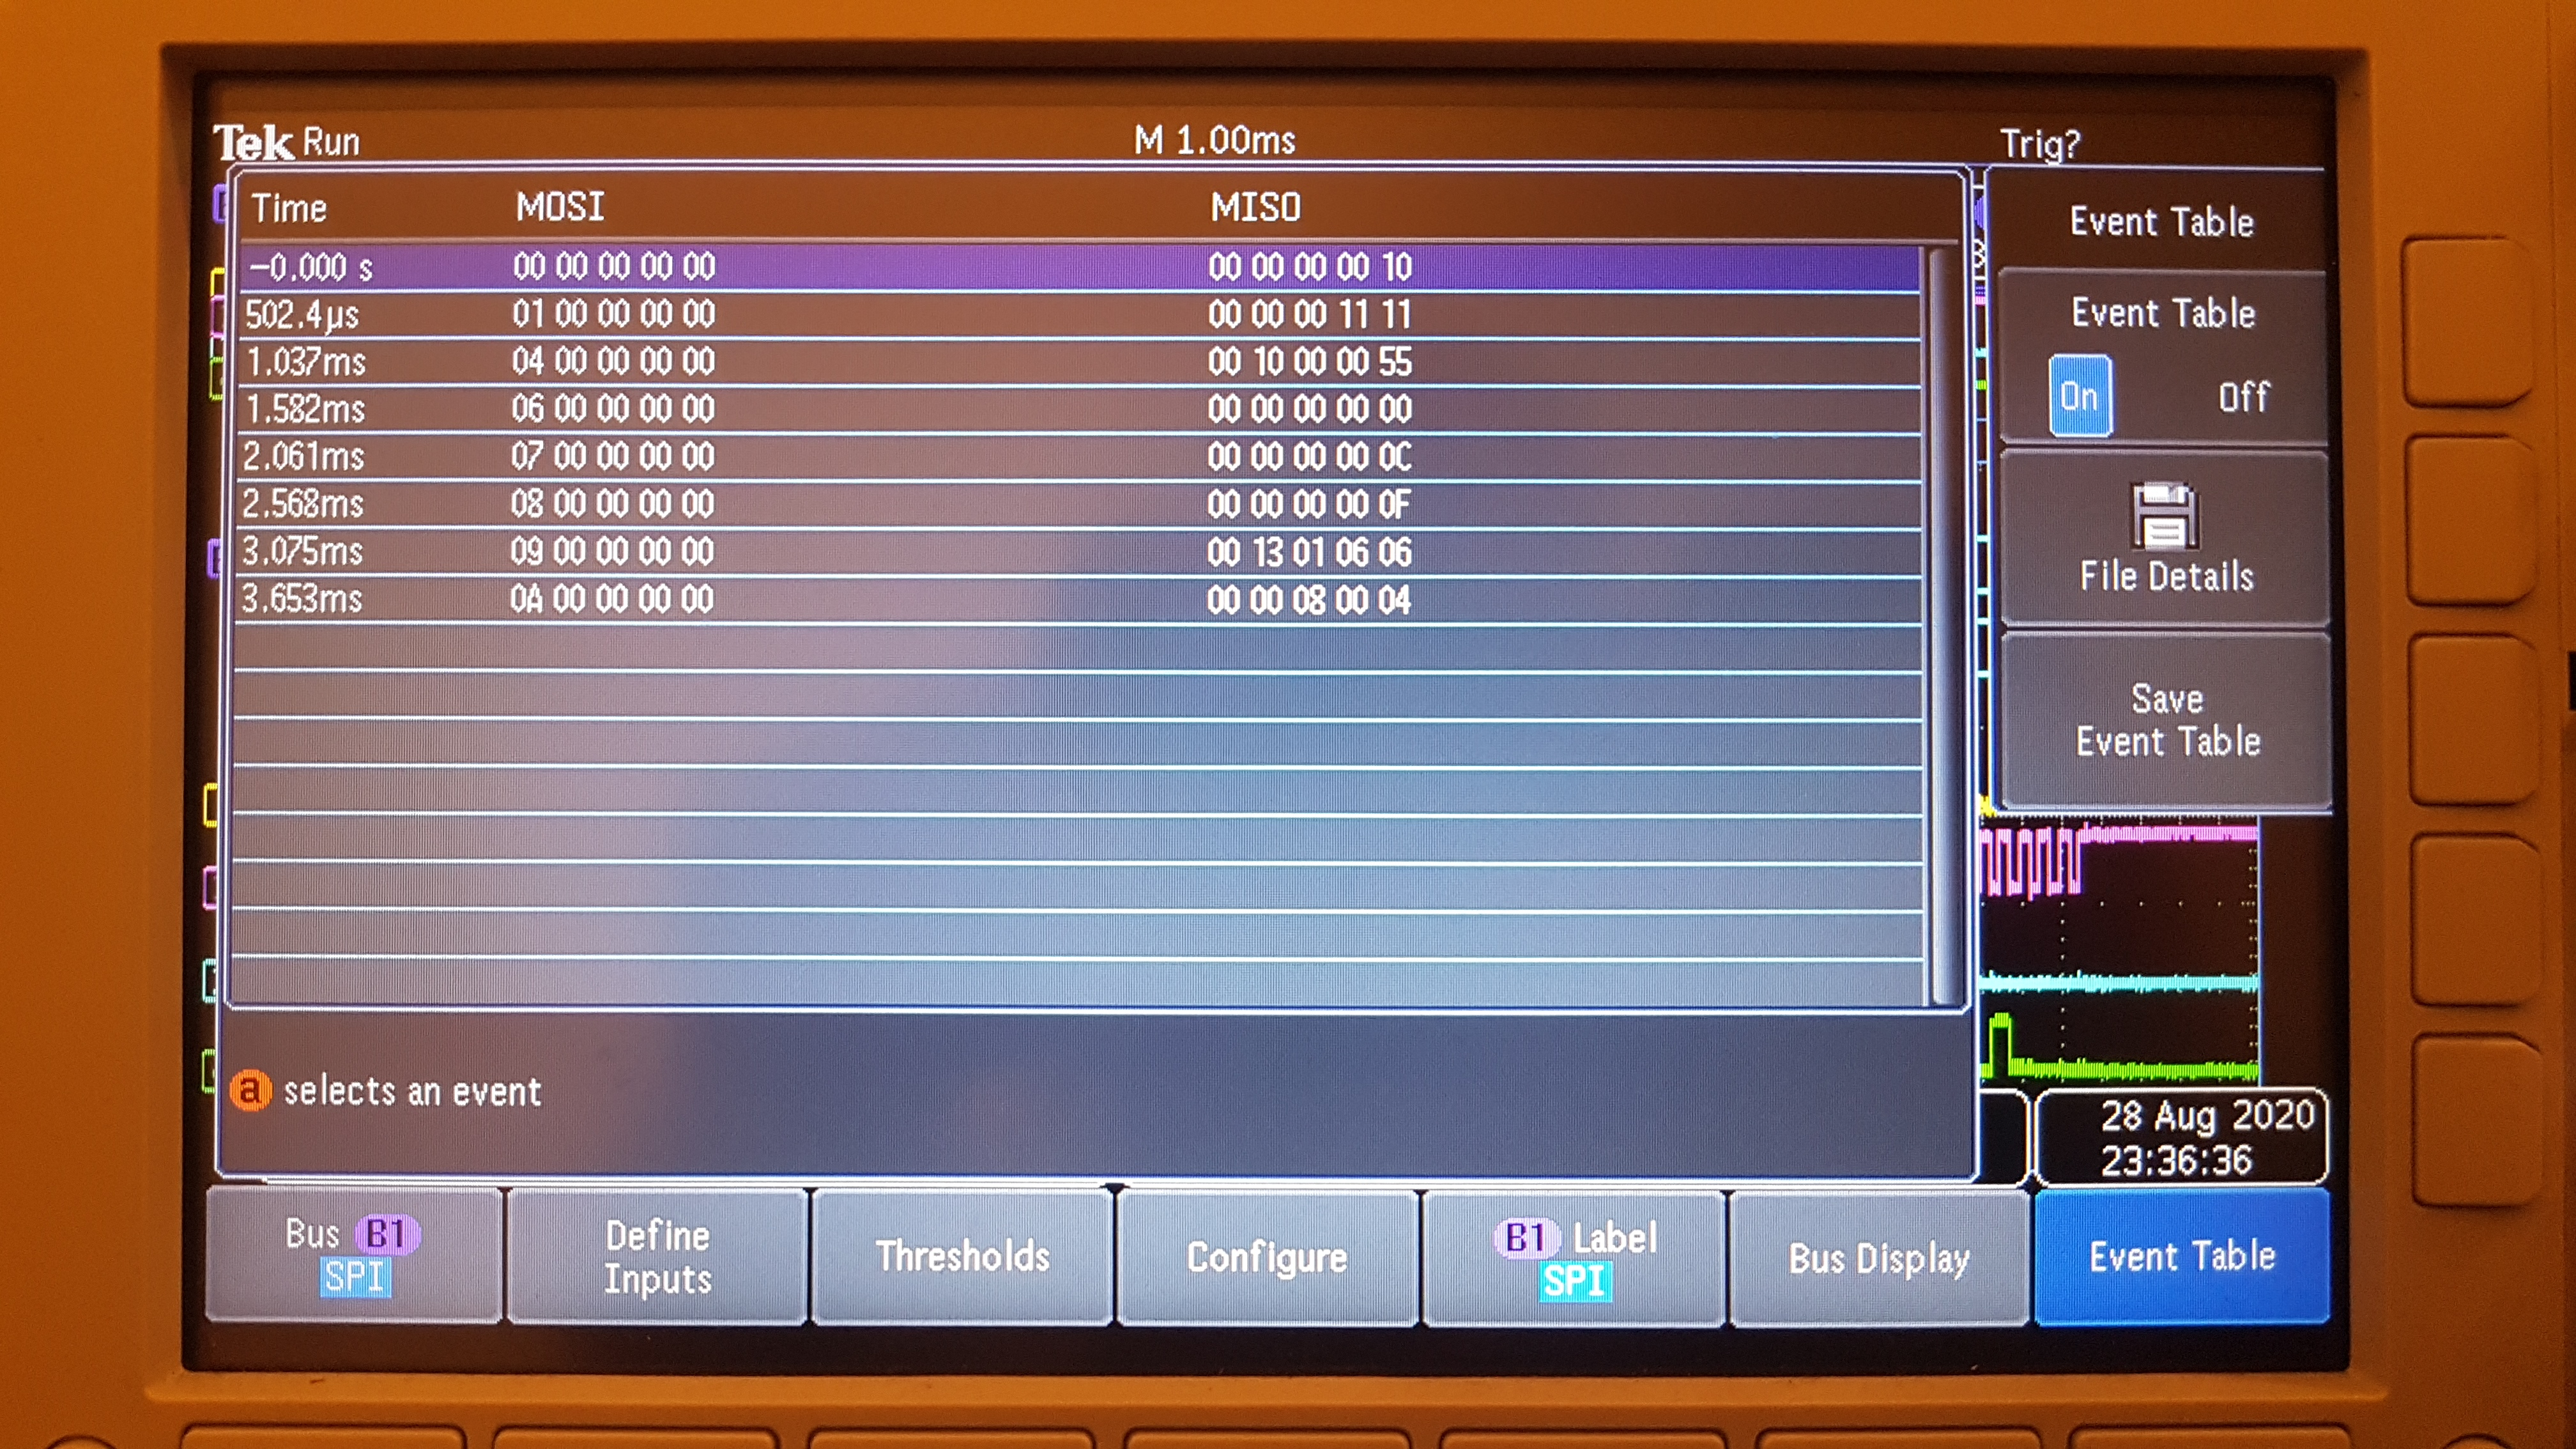
\includegraphics[width = \textwidth]{graphics/TMC6200_EventTable_Lesen_Bild}
\caption{Event-Table Inbetriebnahme TMC6200.}
\label{fig:TMC6200_EventTable_Lesen_Bild}
\end{figure}

\subsubsection{Inbetriebnahme Gate-Ctrl}\label{Appendix:TMC6200_Gate_Ctrl}

\begin{figure}[H]
\center
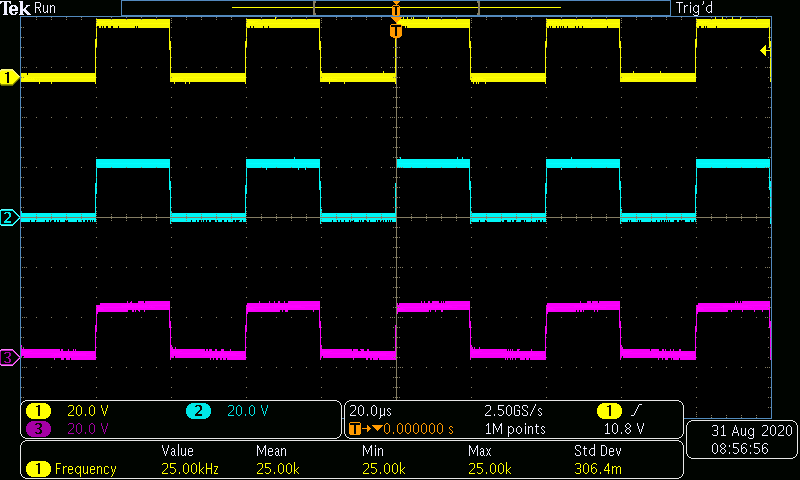
\includegraphics[width = \textwidth]{graphics/TMC6200_Gate_Signal_H}
\caption{Steuersignale PWM 48V von TMC6200 auf H-Brücke. Gelb = U, Blau = V, Magenta = W}
\label{fig:TMC6200_Gate_Signal_H}
\end{figure}

\begin{figure}[H]
\center
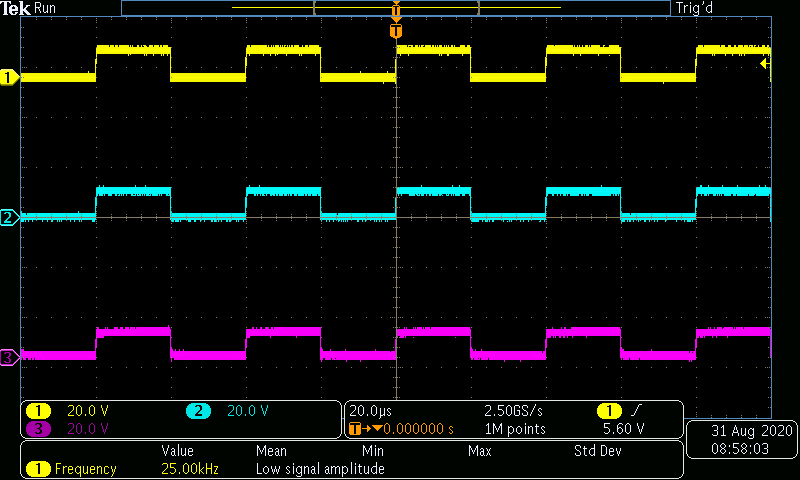
\includegraphics[width = \textwidth]{graphics/TMC6200_Gate_Signal_L}
\caption{Steuersignale PWM 0V von TMC6200 auf H-Brücke. Gelb = U, Blau = V, Magenta = W}
\label{fig:TMC6200_Gate_Signal_L}
\end{figure}